\section{Management of Device Memory}
We have created the template class \texttt{Vector<T>} to represent a vector of elements of type T, where the data is allocated on the device. This class is constructed to follow the idea of Chapter \ref{memoryModelDesign}, where we state that we want the developer to have explicit control of where memory is located. A code snippet with a stripped down version of the class, only showing the relevant content, is shown in Listing \ref{code:memoryManagementVector}, and line number references in this section refer to that listing.

The class contains a device pointer that can be used by the \textit{CUDA} driver API, and a integer to describe the number of elements stored beginning at that address. The lifetime of the object is directly related to the lifetime of the data. When the object is created the necessary allocation is made on the device through the \textit{CUDA} driver API, and when the object is destroyed the allocated data is freed.

To enable data transfers the class is using \textit{STL}s \texttt{vector<T>} to provide a constructor and casting options. The constructor copies data from a \textit{STL} \texttt{vector} to our \texttt{Vector} with \textit{CUDA}s \texttt{memcpy} function as a part of the object initialization, and can be seen at Line \ref{code:memoryManagementVectorConstructors}. To transfer data back we overload the casting operator to a \textit{STL} \texttt{vector}, copying the data from the device to the result \textit{STL} \texttt{vector} as seen at Line \ref{code:memoryManagementVectorCast};

Accessing single data elements are done through get and set functions, as seen at Line \ref{code:memoryManagementVectorAcc}. These functions will perform the needed memory transfer for the user. They are intended only for tasks regarding a single value, as a transfer is needed for every use, and manipulations of the whole vector should be done either in main memory by the CPU, or in device memory by the GPU instead.

To not motivate CPU computations on device memory we chose not to implement an iterator on our \texttt{Vector}. This makes it different from a \textit{STL} \texttt{vector}, but iterating over elements can still be done, by copying the data from the device to a \textit{STL} \texttt{vector}.

\todo{figur der viser data placering måske..}

\todo{resize discussion, let's go?!?}

\begin{lstlisting}[caption={Vector class, showing only code relevant to memory management.}, label={code:memoryManagementVector}, mathescape]
namespace yagal{
    template<typename T>
    class Vector{
    private:
        CUdeviceptr _devicePtr;
        size_t _count;

    public
        // Constructors ~\label{code:memoryManagementVectorConstructors}~
        Vector(int elementCount)
            : _count(elementCount)
        {
            _devicePtr = yagal::cuda::malloc(_count * sizeof(T));
        }

        Vector(const std::vector<T>& source)
            : _count(source.size())
        {
            _devicePtr = yagal::cuda::malloc(_count * sizeof(T));
            yagal::cuda::copyToDevice(_devicePtr, source.data(), _count * sizeof(T));
        }

        // Cast (Copy out) ~\label{code:memoryManagementVectorCast}~
        operator std::vector<T>(){
            std::vector<T> result(_count);
            yagal::cuda::copyToHost(result.data(), _devicePtr, _count * sizeof(T));
            return result;
        }

        // Accessors ~\label{code:memoryManagementVectorAcc}~
        T getElement(int index){
            T result;
            yagal::cuda::copyToHost(&result, _devicePtr + (index * sizeof(T)), sizeof(T));
            return result;
        }

        void setElement(int index, T value){
            yagal::cuda::copyToDevice(_devicePtr + (index * sizeof(T)), &value, sizeof(T));
        }

        // Destructors
        $~$Vector(){
            yagal::cuda::free(_devicePtr);
        }

    }
}
\end{lstlisting}
\todo{fix tilde for destructor i eksempel}

\todo{indsæt kode og referer til linjenumre}

\section{Step 2 - Execute .PTX}
\todo{Brug af CUDA driver API}

\section{Step 3 - Make LLC Replacement}
\todo{Generere PTX fra LLVMIR - Bøvlet - derfor - vores llc erstatning! woo}

\begin{figure}[!htb]
    \centering
    \begin{minipage}{.7\textwidth}
        \centering
        \includegraphics[width=0.9\linewidth]{chapters/implementation/figs/LLVMLLC.png}
        \caption{$dt=0.1$}
        \label{fig:prob1_6_2}
    \end{minipage}%
    \begin{minipage}{0.4\textwidth}
        \centering
        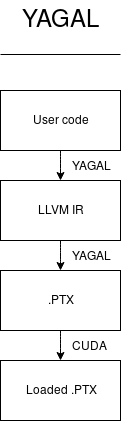
\includegraphics[width=0.5\linewidth]{chapters/implementation/figs/YAGALLLC.png}
        \caption{$dt =$}
        \label{fig:prob1_6_1}
    \end{minipage}
\end{figure}

\section{Step 4 - Generate LLVMIR}
\todo{Lav simpel kernel og brug af vores datatyper}

\section{Step 5 - Multiple functions in one kernel}
\todo{Chaning af functionalitet til en enkelt kernel}

\section{Step 6 - LLVM Optimizations}
\todo{Brug LLVMs erfaring - Det kan betale sig - redegør for det her}

\section{Step 7 - Looping mechanism}
\todo{Behandle data uafhængigt af tråde mængde og input størelse}

\section{Step 8 - Support For Multiple Input Types}
\todo{Support for andre typer end bare floats, så som ints og vectorer}

\section{Final Overview}
\todo{Den "færdige" implementation}